\documentclass[a4paper,11pt]{article}

% ── Packages ──────────────────────────────────────────────────────────────
\usepackage[margin=1in]{geometry}
\usepackage{tikz}
\usetikzlibrary{shapes.geometric, arrows.meta, positioning, fit, backgrounds, calc}
\usepackage{xcolor}
\usepackage{hyperref}
\usepackage{fancyhdr}
\usepackage{titlesec}

% ── Colors ────────────────────────────────────────────────────────────────
\definecolor{done}{HTML}{27AE60}       % Green — completed
\definecolor{inprog}{HTML}{F39C12}     % Amber — in progress
\definecolor{planned}{HTML}{3498DB}    % Blue  — planned/future
\definecolor{sectionbg}{HTML}{ECF0F1}  % Light gray section background
\definecolor{titleblue}{HTML}{2C3E50}  % Dark blue for titles

% ── TikZ Styles ───────────────────────────────────────────────────────────
\tikzset{
    startstop/.style={
        rectangle, rounded corners=6pt, minimum width=3.2cm, minimum height=0.9cm,
        text centered, draw=black!70, line width=0.8pt, font=\small\bfseries
    },
    process/.style={
        rectangle, minimum width=3.5cm, minimum height=0.8cm,
        text centered, draw=black!60, line width=0.6pt, font=\small
    },
    decision/.style={
        diamond, minimum width=2.8cm, minimum height=1cm,
        text centered, draw=black!60, line width=0.6pt, font=\small,
        aspect=2.5
    },
    arrow/.style={
        -Stealth, thick, draw=black!60
    },
    completed/.style={
        fill=done!25, draw=done!70
    },
    inprogress/.style={
        fill=inprog!25, draw=inprog!70
    },
    future/.style={
        fill=planned!20, draw=planned!60
    },
    sectionbox/.style={
        draw=black!30, rounded corners=8pt, fill=sectionbg,
        inner sep=10pt
    }
}

% ── Header/Footer ─────────────────────────────────────────────────────────
\pagestyle{fancy}
\fancyhf{}
\fancyhead[L]{\textcolor{titleblue}{\textbf{FarNav Amiga — Development Progress}}}
\fancyhead[R]{\textcolor{titleblue}{March 2026}}
\fancyfoot[C]{\thepage}
\renewcommand{\headrulewidth}{0.4pt}

% ── Title Formatting ──────────────────────────────────────────────────────
\titleformat{\section}{\Large\bfseries\color{titleblue}}{}{0em}{}
\titleformat{\subsection}{\large\bfseries\color{titleblue!80}}{}{0em}{}

% ══════════════════════════════════════════════════════════════════════════
\begin{document}

\begin{center}
    {\Huge\bfseries\color{titleblue} FarNav Amiga}\\[6pt]
    {\Large Development Progress Flowcharts}\\[4pt]
    {\large Farm-ng Amiga Autonomous Crop-Row Navigation}\\[8pt]
    {\normalsize\color{black!60} Last Updated: March 2026}
\end{center}

\vspace{6pt}

% ── Legend ─────────────────────────────────────────────────────────────────
\begin{center}
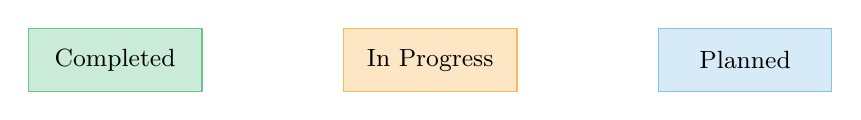
\begin{tikzpicture}
    \node[process, completed, minimum width=2.2cm] at (0,0) {Completed};
    \node[process, inprogress, minimum width=2.2cm] at (4,0) {In Progress};
    \node[process, future, minimum width=2.2cm] at (8,0) {Planned};
\end{tikzpicture}
\end{center}

\vspace{12pt}

% ══════════════════════════════════════════════════════════════════════════
\section{1. gRPC-to-ROS\,2 Bridge}
% ══════════════════════════════════════════════════════════════════════════

\begin{center}
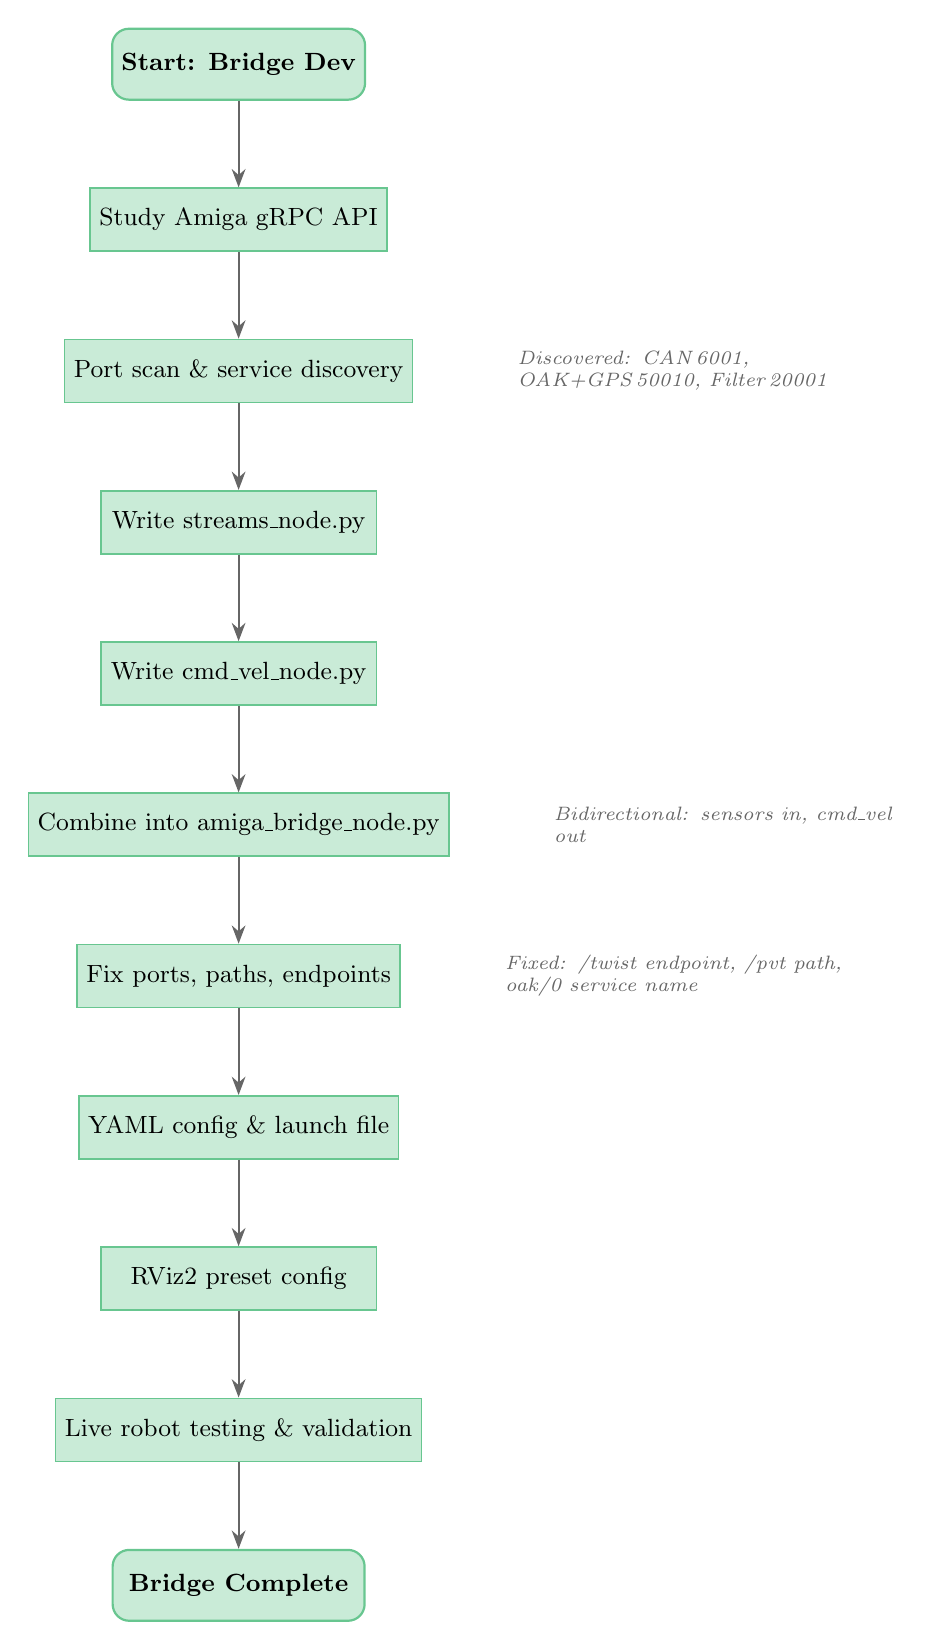
\begin{tikzpicture}[node distance=1.1cm and 0.5cm]

    % ── Nodes ──
    \node[startstop, completed]                        (start)   {Start: Bridge Dev};
    \node[process, completed, below=of start]          (grpc)    {Study Amiga gRPC API};
    \node[process, completed, below=of grpc]           (ports)   {Port scan \& service discovery};
    \node[process, completed, below=of ports]          (proto)   {Write streams\_node.py};
    \node[process, completed, below=of proto]          (cmd)     {Write cmd\_vel\_node.py};
    \node[process, completed, below=of cmd]            (combine) {Combine into amiga\_bridge\_node.py};
    \node[process, completed, below=of combine]        (fix)     {Fix ports, paths, endpoints};
    \node[process, completed, below=of fix]            (config)  {YAML config \& launch file};
    \node[process, completed, below=of config]         (rviz)    {RViz2 preset config};
    \node[process, completed, below=of rviz]           (test)    {Live robot testing \& validation};
    \node[startstop, completed, below=of test]         (done)    {Bridge Complete};

    % ── Arrows ──
    \draw[arrow] (start)   -- (grpc);
    \draw[arrow] (grpc)    -- (ports);
    \draw[arrow] (ports)   -- (proto);
    \draw[arrow] (proto)   -- (cmd);
    \draw[arrow] (cmd)     -- (combine);
    \draw[arrow] (combine) -- (fix);
    \draw[arrow] (fix)     -- (config);
    \draw[arrow] (config)  -- (rviz);
    \draw[arrow] (rviz)    -- (test);
    \draw[arrow] (test)    -- (done);

    % ── Annotations ──
    \node[right=1.2cm of ports, text width=4.5cm, font=\scriptsize\itshape, text=black!60]
        {Discovered: CAN\,6001, OAK+GPS\,50010, Filter\,20001};
    \node[right=1.2cm of fix, text width=4.5cm, font=\scriptsize\itshape, text=black!60]
        {Fixed: /twist endpoint, /pvt path, oak/0 service name};
    \node[right=1.2cm of combine, text width=4.5cm, font=\scriptsize\itshape, text=black!60]
        {Bidirectional: sensors in, cmd\_vel out};

\end{tikzpicture}
\end{center}

\vspace{8pt}

% ══════════════════════════════════════════════════════════════════════════
\section{2. Global Path Planner}
% ══════════════════════════════════════════════════════════════════════════

\begin{center}
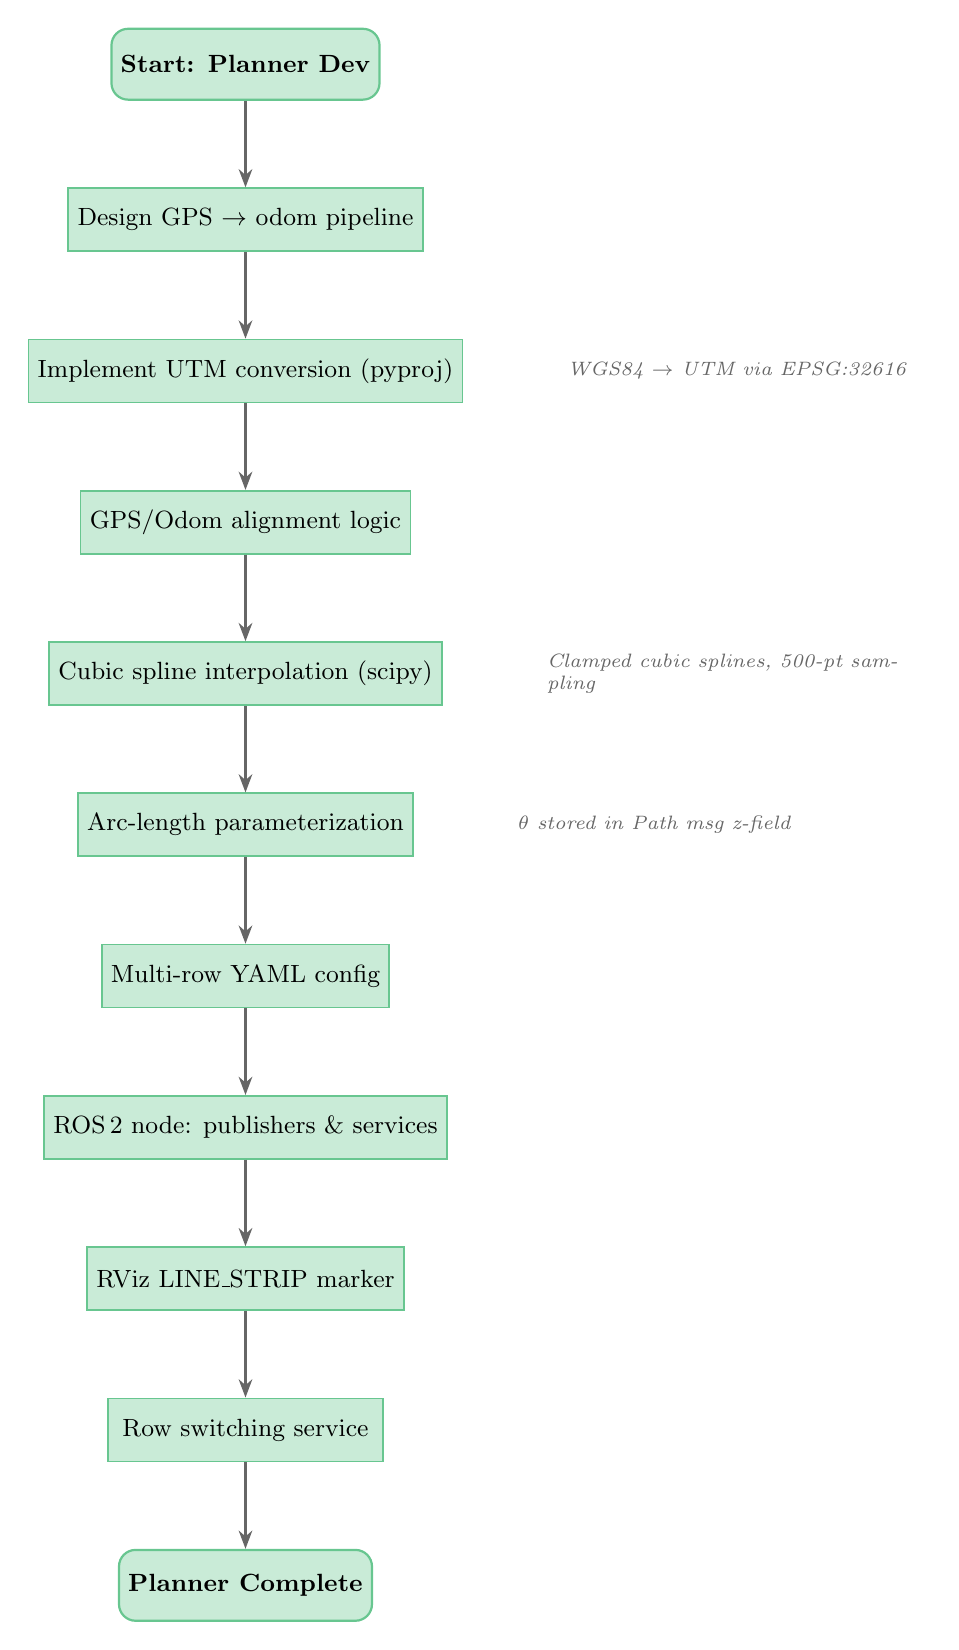
\begin{tikzpicture}[node distance=1.1cm and 0.5cm]

    \node[startstop, completed]                         (start)    {Start: Planner Dev};
    \node[process, completed, below=of start]           (design)   {Design GPS $\to$ odom pipeline};
    \node[process, completed, below=of design]          (utm)      {Implement UTM conversion (pyproj)};
    \node[process, completed, below=of utm]             (align)    {GPS/Odom alignment logic};
    \node[process, completed, below=of align]           (spline)   {Cubic spline interpolation (scipy)};
    \node[process, completed, below=of spline]          (arclength){Arc-length parameterization};
    \node[process, completed, below=of arclength]       (yaml)     {Multi-row YAML config};
    \node[process, completed, below=of yaml]            (ros)      {ROS\,2 node: publishers \& services};
    \node[process, completed, below=of ros]             (marker)   {RViz LINE\_STRIP marker};
    \node[process, completed, below=of marker]          (rowswitch){Row switching service};
    \node[startstop, completed, below=of rowswitch]     (done)     {Planner Complete};

    \draw[arrow] (start)     -- (design);
    \draw[arrow] (design)    -- (utm);
    \draw[arrow] (utm)       -- (align);
    \draw[arrow] (align)     -- (spline);
    \draw[arrow] (spline)    -- (arclength);
    \draw[arrow] (arclength) -- (yaml);
    \draw[arrow] (yaml)      -- (ros);
    \draw[arrow] (ros)       -- (marker);
    \draw[arrow] (marker)    -- (rowswitch);
    \draw[arrow] (rowswitch) -- (done);

    \node[right=1.2cm of utm, text width=4.5cm, font=\scriptsize\itshape, text=black!60]
        {WGS84 $\to$ UTM via EPSG:32616};
    \node[right=1.2cm of spline, text width=4.5cm, font=\scriptsize\itshape, text=black!60]
        {Clamped cubic splines, 500-pt sampling};
    \node[right=1.2cm of arclength, text width=4.5cm, font=\scriptsize\itshape, text=black!60]
        {$\theta$ stored in Path msg z-field};

\end{tikzpicture}
\end{center}

\newpage

% ══════════════════════════════════════════════════════════════════════════
\section{3. MPC Controller}
% ══════════════════════════════════════════════════════════════════════════

\begin{center}
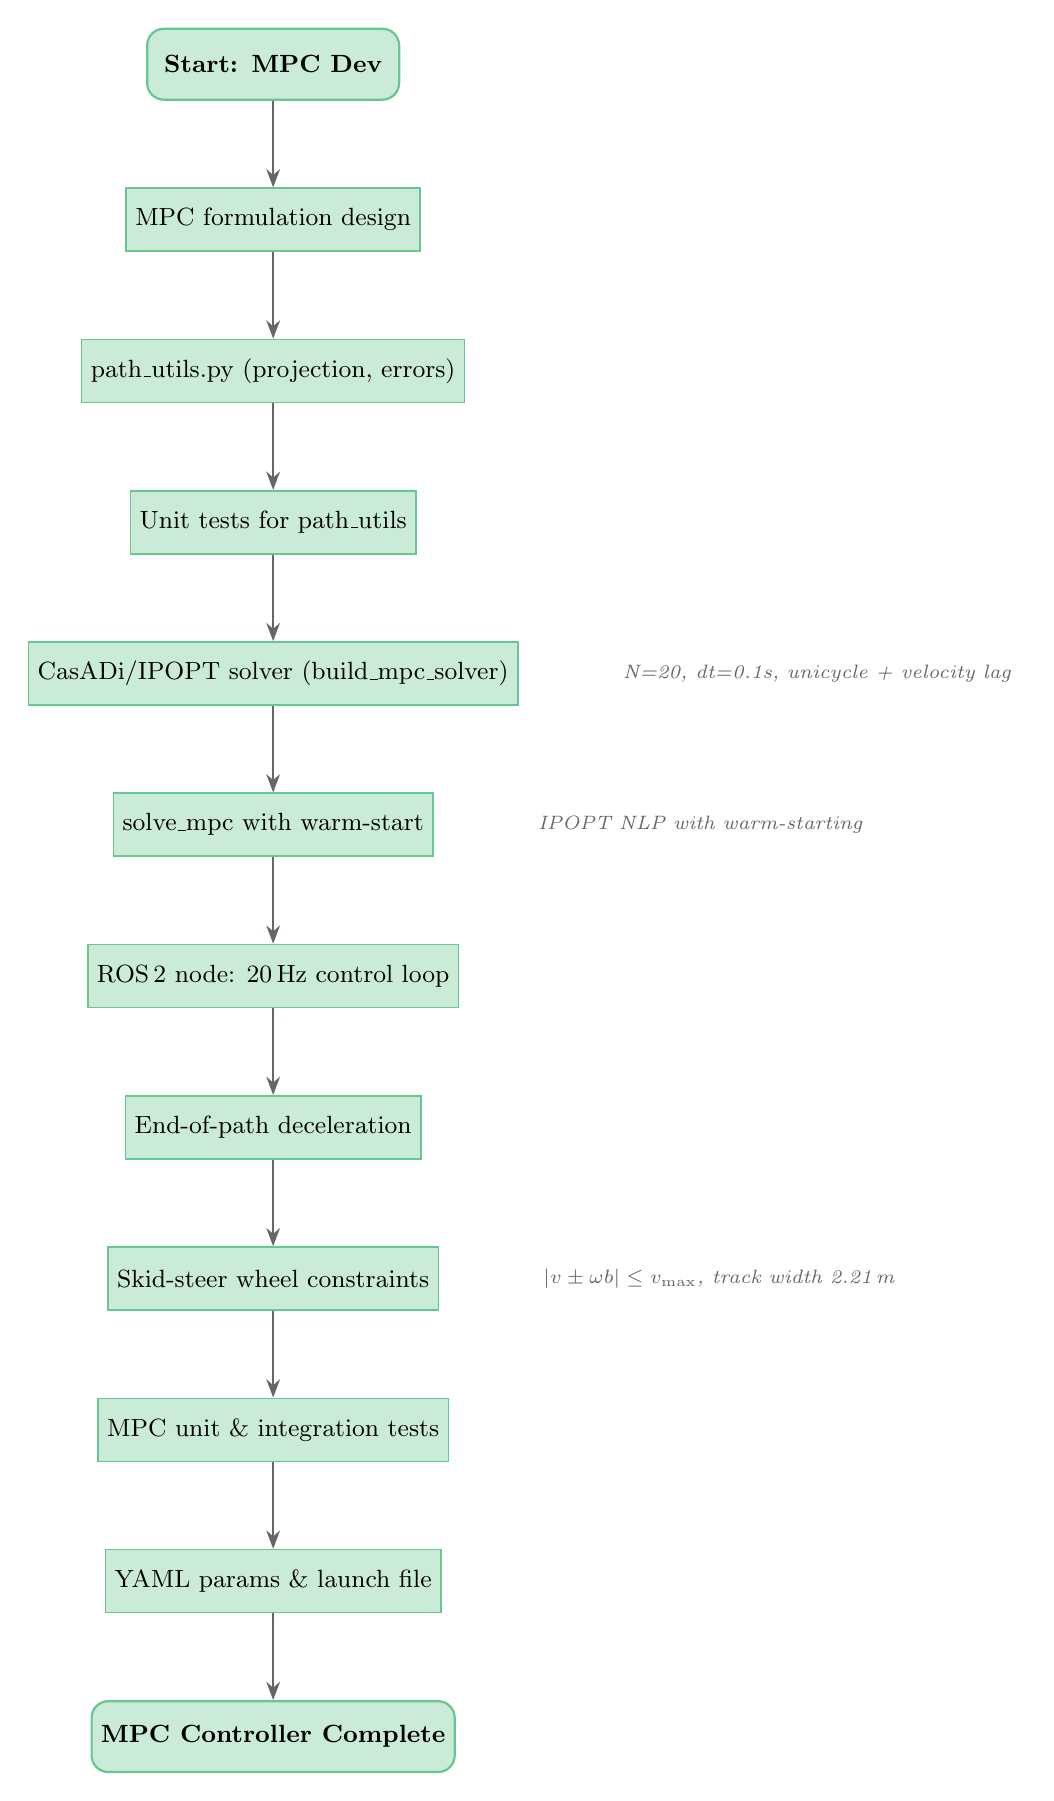
\begin{tikzpicture}[node distance=1.1cm and 0.5cm]

    \node[startstop, completed]                         (start)    {Start: MPC Dev};
    \node[process, completed, below=of start]           (design)   {MPC formulation design};
    \node[process, completed, below=of design]          (pathutil) {path\_utils.py (projection, errors)};
    \node[process, completed, below=of pathutil]        (testp)    {Unit tests for path\_utils};
    \node[process, completed, below=of testp]           (casadi)   {CasADi/IPOPT solver (build\_mpc\_solver)};
    \node[process, completed, below=of casadi]          (solve)    {solve\_mpc with warm-start};
    \node[process, completed, below=of solve]           (node)     {ROS\,2 node: 20\,Hz control loop};
    \node[process, completed, below=of node]            (decel)    {End-of-path deceleration};
    \node[process, completed, below=of decel]           (constr)   {Skid-steer wheel constraints};
    \node[process, completed, below=of constr]          (testm)    {MPC unit \& integration tests};
    \node[process, completed, below=of testm]           (yaml)     {YAML params \& launch file};
    \node[startstop, completed, below=of yaml]          (done)     {MPC Controller Complete};

    \draw[arrow] (start)    -- (design);
    \draw[arrow] (design)   -- (pathutil);
    \draw[arrow] (pathutil) -- (testp);
    \draw[arrow] (testp)    -- (casadi);
    \draw[arrow] (casadi)   -- (solve);
    \draw[arrow] (solve)    -- (node);
    \draw[arrow] (node)     -- (decel);
    \draw[arrow] (decel)    -- (constr);
    \draw[arrow] (constr)   -- (testm);
    \draw[arrow] (testm)    -- (yaml);
    \draw[arrow] (yaml)     -- (done);

    \node[right=1.2cm of casadi, text width=5cm, font=\scriptsize\itshape, text=black!60]
        {N=20, dt=0.1s, unicycle + velocity lag};
    \node[right=1.2cm of solve, text width=5cm, font=\scriptsize\itshape, text=black!60]
        {IPOPT NLP with warm-starting};
    \node[right=1.2cm of constr, text width=5cm, font=\scriptsize\itshape, text=black!60]
        {$|v \pm \omega b| \leq v_{\max}$, track width 2.21\,m};

\end{tikzpicture}
\end{center}

\vspace{8pt}

% ══════════════════════════════════════════════════════════════════════════
\section{4. Testing \& Validation}
% ══════════════════════════════════════════════════════════════════════════

\begin{center}
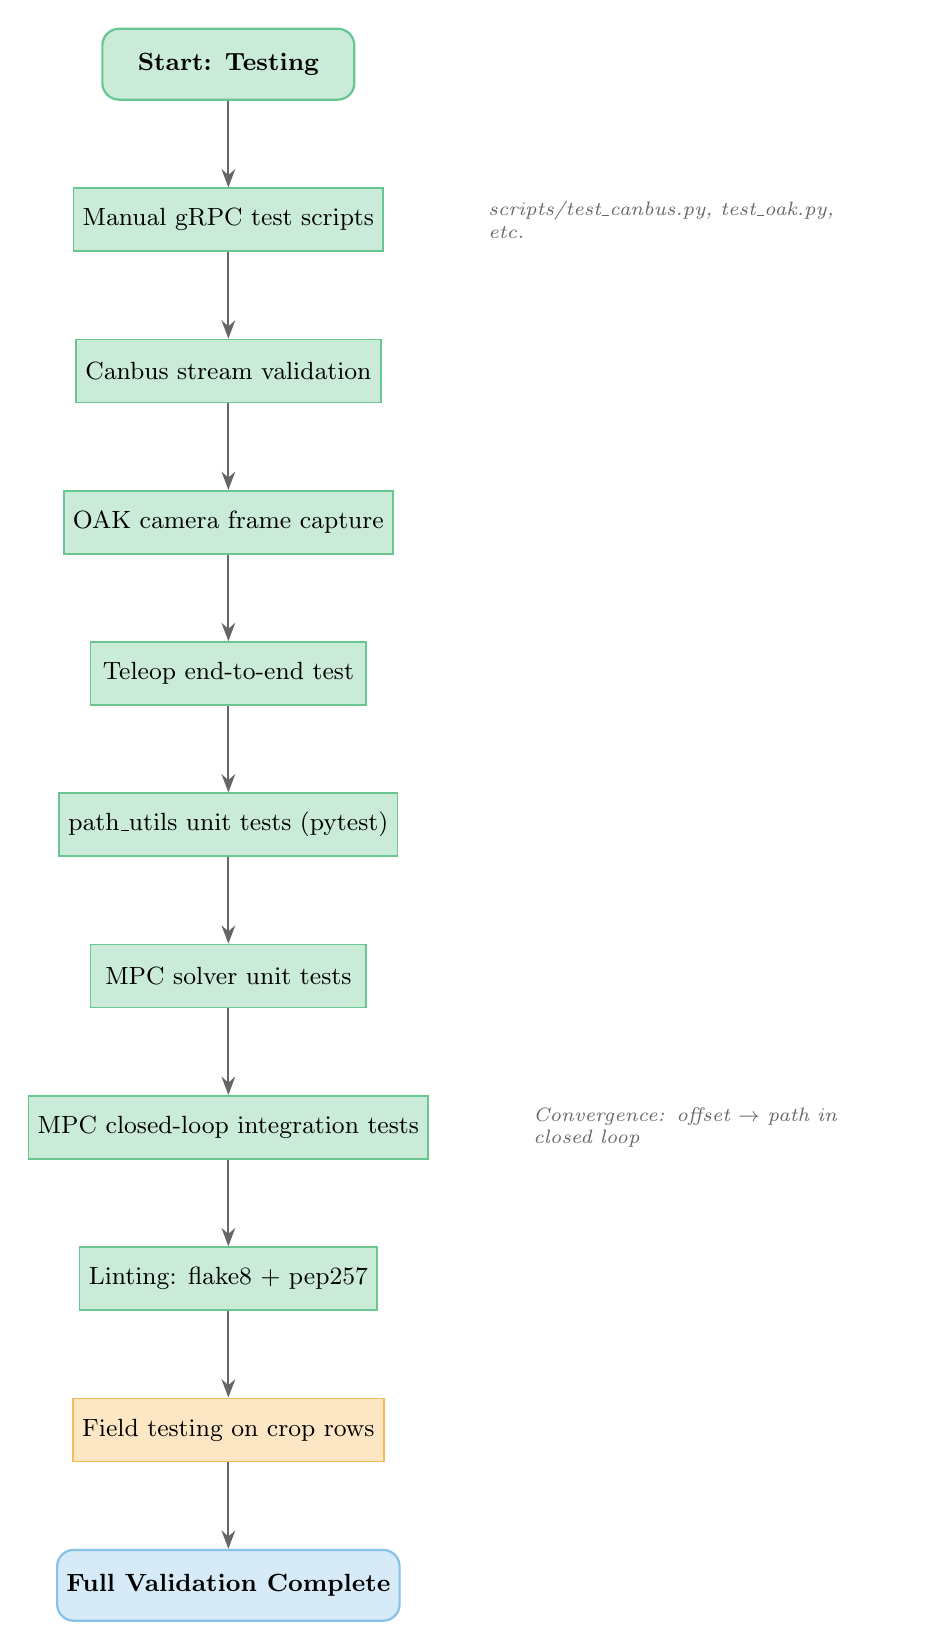
\begin{tikzpicture}[node distance=1.1cm and 0.5cm]

    \node[startstop, completed]                         (start)   {Start: Testing};
    \node[process, completed, below=of start]           (manual)  {Manual gRPC test scripts};
    \node[process, completed, below=of manual]          (canbus)  {Canbus stream validation};
    \node[process, completed, below=of canbus]          (oak)     {OAK camera frame capture};
    \node[process, completed, below=of oak]             (teleop)  {Teleop end-to-end test};
    \node[process, completed, below=of teleop]          (upath)   {path\_utils unit tests (pytest)};
    \node[process, completed, below=of upath]           (umpc)    {MPC solver unit tests};
    \node[process, completed, below=of umpc]            (integ)   {MPC closed-loop integration tests};
    \node[process, completed, below=of integ]           (lint)    {Linting: flake8 + pep257};
    \node[process, inprogress, below=of lint]           (field)   {Field testing on crop rows};
    \node[startstop, future, below=of field]            (done)    {Full Validation Complete};

    \draw[arrow] (start)  -- (manual);
    \draw[arrow] (manual) -- (canbus);
    \draw[arrow] (canbus) -- (oak);
    \draw[arrow] (oak)    -- (teleop);
    \draw[arrow] (teleop) -- (upath);
    \draw[arrow] (upath)  -- (umpc);
    \draw[arrow] (umpc)   -- (integ);
    \draw[arrow] (integ)  -- (lint);
    \draw[arrow] (lint)   -- (field);
    \draw[arrow] (field)  -- (done);

    \node[right=1.2cm of manual, text width=4.5cm, font=\scriptsize\itshape, text=black!60]
        {scripts/test\_canbus.py, test\_oak.py, etc.};
    \node[right=1.2cm of integ, text width=4.5cm, font=\scriptsize\itshape, text=black!60]
        {Convergence: offset $\to$ path in closed loop};

\end{tikzpicture}
\end{center}

\newpage

% ══════════════════════════════════════════════════════════════════════════
\section{5. Visualization \& Utilities}
% ══════════════════════════════════════════════════════════════════════════

\begin{center}
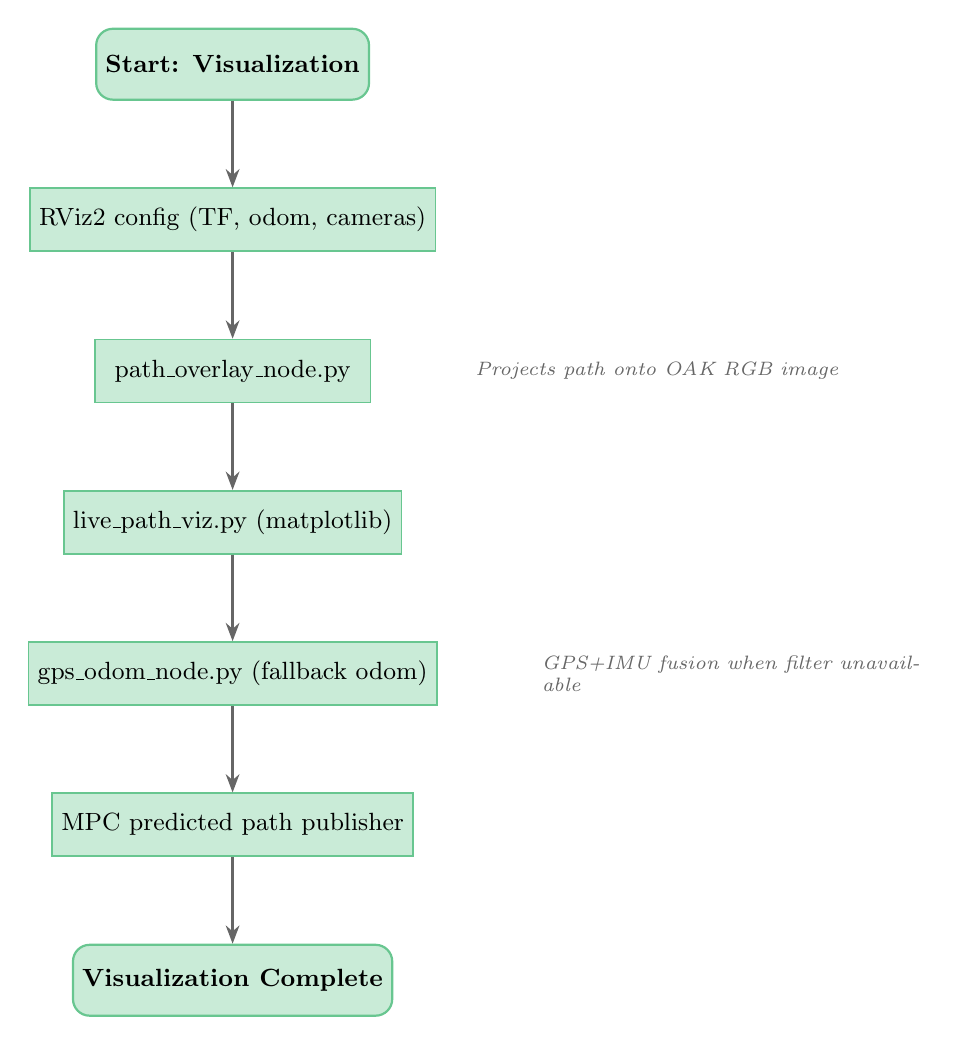
\begin{tikzpicture}[node distance=1.1cm and 0.5cm]

    \node[startstop, completed]                         (start)   {Start: Visualization};
    \node[process, completed, below=of start]           (rviz)    {RViz2 config (TF, odom, cameras)};
    \node[process, completed, below=of rviz]            (overlay) {path\_overlay\_node.py};
    \node[process, completed, below=of overlay]         (live)    {live\_path\_viz.py (matplotlib)};
    \node[process, completed, below=of live]            (gpsodom) {gps\_odom\_node.py (fallback odom)};
    \node[process, completed, below=of gpsodom]         (mpcviz)  {MPC predicted path publisher};
    \node[startstop, completed, below=of mpcviz]        (done)    {Visualization Complete};

    \draw[arrow] (start)   -- (rviz);
    \draw[arrow] (rviz)    -- (overlay);
    \draw[arrow] (overlay) -- (live);
    \draw[arrow] (live)    -- (gpsodom);
    \draw[arrow] (gpsodom) -- (mpcviz);
    \draw[arrow] (mpcviz)  -- (done);

    \node[right=1.2cm of overlay, text width=5cm, font=\scriptsize\itshape, text=black!60]
        {Projects path onto OAK RGB image};
    \node[right=1.2cm of gpsodom, text width=5cm, font=\scriptsize\itshape, text=black!60]
        {GPS+IMU fusion when filter unavailable};

\end{tikzpicture}
\end{center}

\vspace{8pt}

% ══════════════════════════════════════════════════════════════════════════
\section{6. Documentation \& Repository}
% ══════════════════════════════════════════════════════════════════════════

\begin{center}
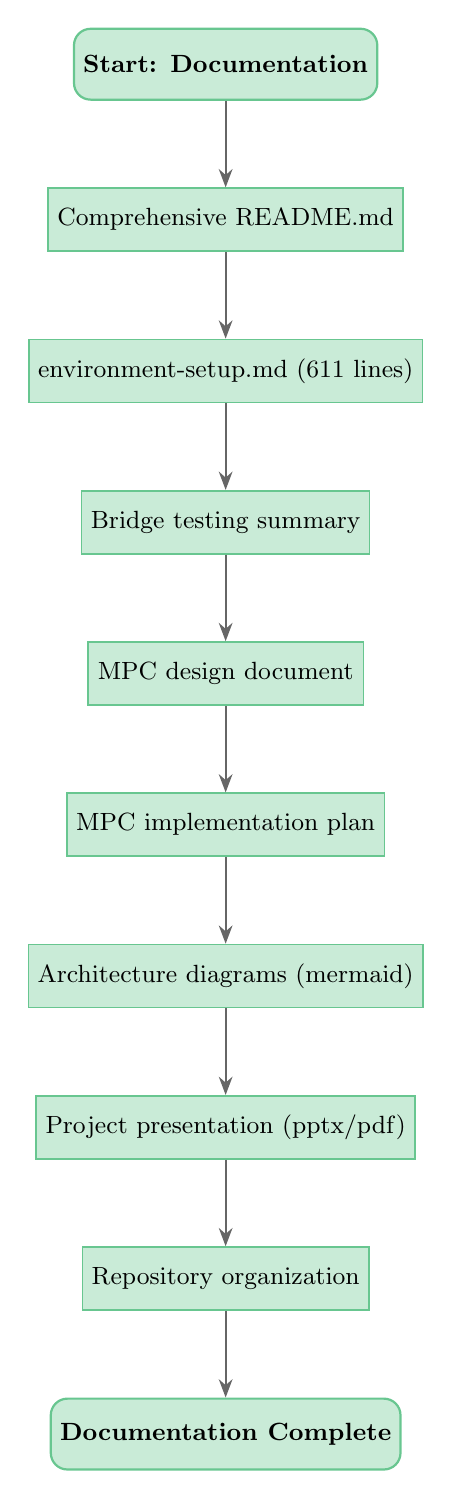
\begin{tikzpicture}[node distance=1.1cm and 0.5cm]

    \node[startstop, completed]                         (start)   {Start: Documentation};
    \node[process, completed, below=of start]           (readme)  {Comprehensive README.md};
    \node[process, completed, below=of readme]          (setup)   {environment-setup.md (611 lines)};
    \node[process, completed, below=of setup]           (testing) {Bridge testing summary};
    \node[process, completed, below=of testing]         (design)  {MPC design document};
    \node[process, completed, below=of design]          (plan)    {MPC implementation plan};
    \node[process, completed, below=of plan]            (arch)    {Architecture diagrams (mermaid)};
    \node[process, completed, below=of arch]            (pptx)    {Project presentation (pptx/pdf)};
    \node[process, completed, below=of pptx]            (reorg)   {Repository organization};
    \node[startstop, completed, below=of reorg]         (done)    {Documentation Complete};

    \draw[arrow] (start)   -- (readme);
    \draw[arrow] (readme)  -- (setup);
    \draw[arrow] (setup)   -- (testing);
    \draw[arrow] (testing) -- (design);
    \draw[arrow] (design)  -- (plan);
    \draw[arrow] (plan)    -- (arch);
    \draw[arrow] (arch)    -- (pptx);
    \draw[arrow] (pptx)    -- (reorg);
    \draw[arrow] (reorg)   -- (done);

\end{tikzpicture}
\end{center}

\vspace{8pt}

% ══════════════════════════════════════════════════════════════════════════
\section{7. Overall Project Progress}
% ══════════════════════════════════════════════════════════════════════════

\begin{center}
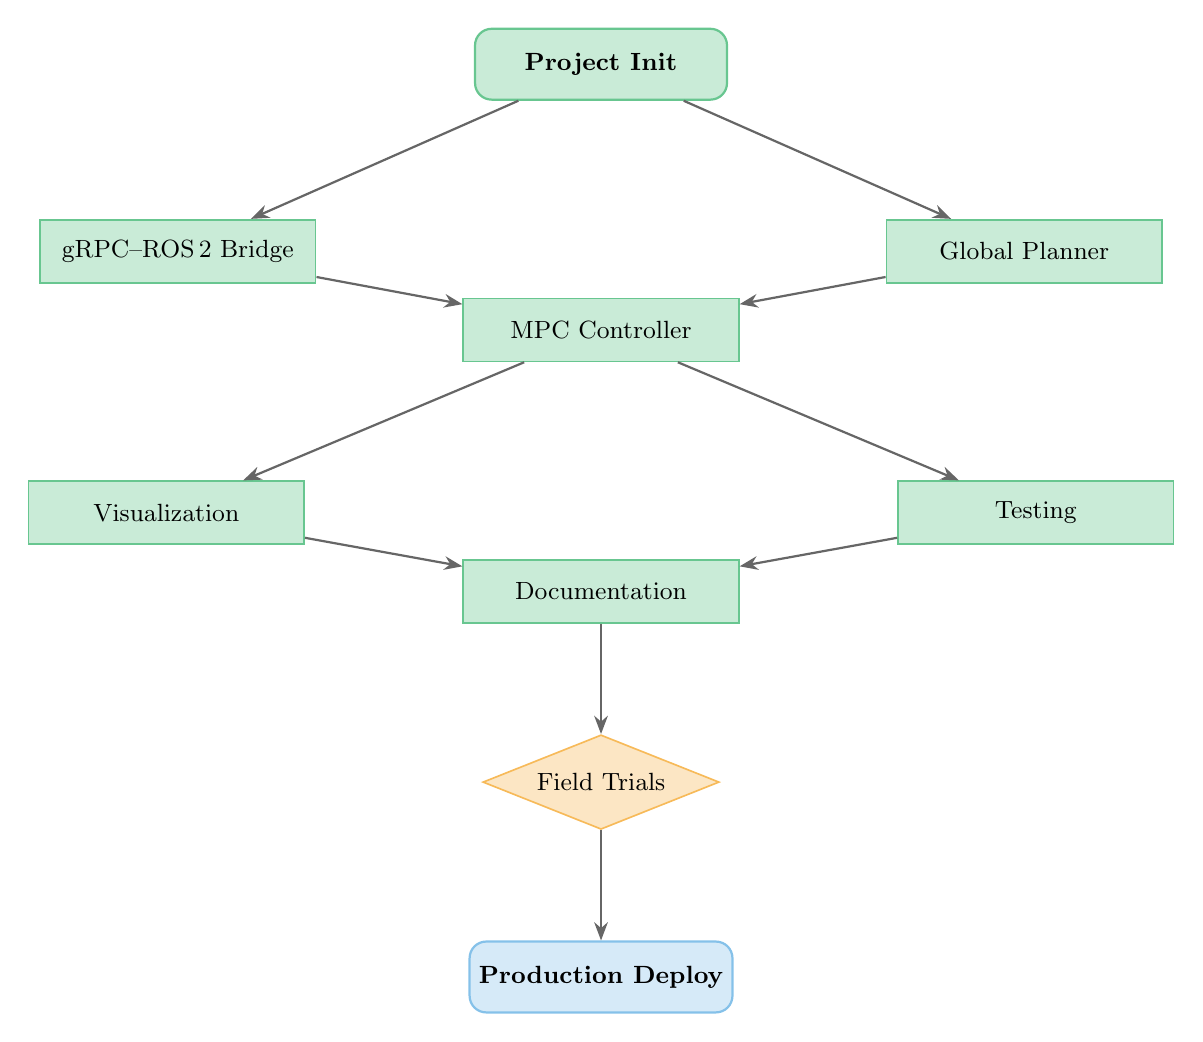
\begin{tikzpicture}[node distance=1.4cm and 2.5cm]

    % ── Top level flow ──
    \node[startstop, completed]                           (init)    {Project Init};

    \node[process, completed, below left=1.5cm and 2cm of init]   (bridge)  {gRPC--ROS\,2 Bridge};
    \node[process, completed, below right=1.5cm and 2cm of init]  (planner) {Global Planner};

    \node[process, completed, below=2.5cm of init]                (mpc)     {MPC Controller};

    \node[process, completed, below left=1.5cm and 2cm of mpc]   (viz)     {Visualization};
    \node[process, completed, below right=1.5cm and 2cm of mpc]  (tests)   {Testing};

    \node[process, completed, below=2.5cm of mpc]                (docs)    {Documentation};

    \node[decision, inprogress, below=of docs]                    (field)   {Field Trials};

    \node[startstop, future, below=of field]                      (deploy)  {Production Deploy};

    % ── Arrows ──
    \draw[arrow] (init)    -- (bridge);
    \draw[arrow] (init)    -- (planner);
    \draw[arrow] (bridge)  -- (mpc);
    \draw[arrow] (planner) -- (mpc);
    \draw[arrow] (mpc)     -- (viz);
    \draw[arrow] (mpc)     -- (tests);
    \draw[arrow] (viz)     -- (docs);
    \draw[arrow] (tests)   -- (docs);
    \draw[arrow] (docs)    -- (field);
    \draw[arrow] (field)   -- (deploy);

\end{tikzpicture}
\end{center}

\vspace{12pt}

% ── Summary Table ─────────────────────────────────────────────────────────
\section{Progress Summary}

\begin{center}
\renewcommand{\arraystretch}{1.3}
\begin{tabular}{|l|c|c|l|}
\hline
\textbf{Section} & \textbf{Status} & \textbf{Completion} & \textbf{Key Deliverable} \\
\hline
gRPC--ROS\,2 Bridge      & \textcolor{done}{\textbf{Done}}      & 100\% & amiga\_bridge\_node.py \\
Global Path Planner       & \textcolor{done}{\textbf{Done}}      & 100\% & global\_planner.py \\
MPC Controller            & \textcolor{done}{\textbf{Done}}      & 100\% & controller\_mpc.py \\
Testing (unit/integration)& \textcolor{done}{\textbf{Done}}      & 100\% & pytest suite \\
Visualization             & \textcolor{done}{\textbf{Done}}      & 100\% & RViz + overlay nodes \\
Documentation             & \textcolor{done}{\textbf{Done}}      & 100\% & README + setup guide \\
Field Testing             & \textcolor{inprog}{\textbf{Active}}  &  50\% & On-robot validation \\
Production Deploy         & \textcolor{planned}{\textbf{Planned}} &   0\% & Autonomous operation \\
\hline
\end{tabular}
\end{center}

\end{document}
